\documentclass[12pt,a4paper,ngerman]{article}
\usepackage[utf8]{inputenc}
\usepackage[ngerman]{babel}
\usepackage{csquotes}
\MakeOuterQuote{"}

\usepackage{fancyref}
\usepackage{fancyhdr}
\usepackage{xcolor}
\usepackage{url}
\usepackage{makeidx}
\usepackage{listings}

% for using text in equations like \frac{\text{...}{\text{....}
\usepackage{amsmath}

% PDF settings
\usepackage[pdftex]{graphicx}
\usepackage[pdfstartview=FitH,pdftitle={Parallelisierte Visualisierung der Schwingung einer Gitarrensaite auf Grundlage der Wellengleichung mit OpenMP und OpenMPI},pdfauthor={Patrick Fehling \& Christian Schütt},
colorlinks=false, linktocpage]{hyperref}
\usepackage[a4paper,includeheadfoot,left=2.6cm,right=2.6cm,top=2.54cm,bottom=2.54cm]{geometry}
\usepackage{array}
\setlength\extrarowheight{5pt}

\usepackage[nottoc,numbib]{tocbibind}
\usepackage{hyperref}
\usepackage{caption}

\usepackage{tabularx}
\newcolumntype{L}[1]{>{\raggedright\arraybackslash}p{#1}} % linksbündig mit Breitenangabe
\newcolumntype{C}[1]{>{\centering\arraybackslash}p{#1}} % zentriert mit Breitenangabe
\newcolumntype{R}[1]{>{\raggedleft\arraybackslash}p{#1}} % rechtsbündig mit Breitenangabe

%for e.g. average symbol
\usepackage{amssymb}
\usepackage{float}

%for cycle schemes
\usepackage{smartdiagram}

%for e.g. bar chart
\usepackage{pgfplots}

% Header and Footer Style
\pagestyle{fancy}
\fancyhead{}
\fancyhead[R]{\slshape Patrick Fehling \& Christian Schütt}
\fancyhead[L]{\slshape\nouppercase{\rightmark}}
\fancyfoot{}
\fancyfoot[C]{\thepage}
\renewcommand{\headrulewidth}{0pt}
\renewcommand{\sectionmark}[1]{\markright{\thesection\ #1}}
\renewcommand{\subsectionmark}[1]{} %Remove \subsection from header

% No identation
\setlength\headheight{15pt}
\setlength\parindent{0pt}

% Custom commands
\newcommand\zb{z.\,B.\ }
\renewcommand\dh{d.\,h.\ }
\newcommand\parbig{\par\bigskip}
\newcommand\parmed{\par\medskip}
\newcommand{\mailto}[1]{\href{mailto:#1}{#1}}

% Java Code Listing Style
\definecolor{darkblue}{rgb}{0,0,.6}
\definecolor{darkgreen}{rgb}{0,0.5,0}
\definecolor{darkred}{rgb}{0.5,0,0}

\lstset{basicstyle=\ttfamily\footnotesize\upshape, commentstyle=\color{darkgreen}\sffamily, keywordstyle=\color{darkblue}\rmfamily\bfseries, breaklines=true, tabsize=2, xleftmargin=3mm,
xrightmargin=3mm, stringstyle=\color{darkred}, showstringspaces=false}

\begin{document}

\begin{titlepage}
\thispagestyle{empty}

\begin{center}
	
\includegraphics[width=0.6\textwidth]{pictures/HTW_Logo}
	
	\vspace{2cm}
	
	\Huge 
	Parallelisierte Visualisierung der Schwingung einer Gitarrensaite auf Grundlage der Wellengleichung mit OpenMP und OpenMPI
	
	\vspace{2cm}
	\large
	Projekt im Fach "Parallel Systems"
	
	\vspace{2cm}
	
	Prüfer: Sebastian Bauer
	
	\vspace{0.5cm}
	
	Eingereicht von Patrick Fehling und Christian Schütt
	
	\vspace{0.5cm}
	
	\today
\end{center}


\end{titlepage}

\pagestyle{empty}

\tableofcontents
\setcounter{page}{0}

\clearpage\pagenumbering{arabic}
\pagestyle{fancy}

% !TEX root = main.tex

\section{Einleitung}
\subsection{Projektzielstellung}
Die zu erfüllende Aufgabe dieses Projektes war es die Amplituden einer vibrierenden Saite auf Grundlage der Wellengleichung im eindimensionalen Fall zu visualisieren. Eine Approximation hierfür bildet die folgende Gleichung:
\begin{quote}
	$A(i, t + 1) = 2A(i, t) - A(i, t - 1) + c(A(i - 1, t) - 2A(i, t) + A(i + 1, t))$
\end{quote}

Neben einer sequentiellen Berechnung der Visualisierung sollten auch zwei unterschiedliche Frameworks verwendet werden, welche die Rechenkraft mehrerer Prozessorkerne oder Grafikprozessoren in Anspruch nehmen. Ein mögliches Aussehen einer so berechneten Kurve ist in Abbildung \ref{fig:example_wave} zu sehen.\\
\begin{figure}[H]
	\centering
	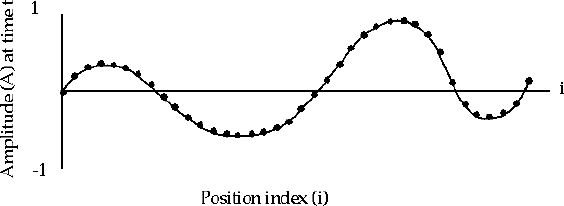
\includegraphics[width=1\textwidth]{pictures/wellengleichung_aufgabe}
	\caption{Schwingung einer Gitarrensaite}
	\label{fig:example_wave}
\end{figure}

Weitere Rahmenbedingungen waren:
\begin{itemize}
	\item Graphical User Interface (Benutzeroberfläche)
	\item Konfiguration per Benutzeroberfläche oder Konfigurationsdatei
	\item Performancevergleich der verschiedenen Varianten
	\item Zwischenpräsentation der Ergebnisse
	\item Paper zum endgültigen Ergebnis
	\item Quellcode-Dokumentation
\end{itemize}

\subsection{Aufbau der Arbeit}
Gegenstand dieser Arbeit sind die Ergebnisse des Projektes und der Weg dorthin. Dies beinhaltet insbesondere den Performancevergleich und die Benutzung der Programme (siehe Rahmenbedingungen).\\
In dieser Arbeit werden zunächst einige Grundlagen zur hier verwendeten Parallelisierung und zu den verwendeten Frameworks erläutert. Des Weiteren gehen wir oberflächlich auf die mathematischen Hintergründe der Aufgabe ein.\\
Anschließend wird die Struktur und der Ablauf unserer drei Programme und wie dieser umgesetzt wurde dargestellt. Schließlich wird gezeigt wie die Anwendungen getestet wurden und zu welchen Schlussfolgerungen wir gekommen sind.
% !TEX root = main.tex

\section{Grundlagen}

\subsection{Wellengleichung}\label{sec:wave_equation}
%TODO: Überarbeiten --> zweite Gleichung rausnehmen und als Text schreiben
Die Basis der zu entwickelnden Programme bildet folgende Gleichung:
\begin{quote}
	$A(i, t + 1) = 2A(i, t) - A(i, t - 1) + c(A(i - 1, t) - 2A(i, t) + A(i + 1, t))$
\end{quote}
Dabei ist $t$ der Zeitpunkt Schwingung, $i$ der Index der Welle und A(i,t) steht für die Amplitude zum Zeitpunkt t und am Punkt i.\\
Klarer wird diese wenn man sich A(i, t+1), also das Ergebnis der Gleichung, als den zukünftigen Wert an der aktuellen Stelle (futureVal) vorstellt. Dann würde die Gleichung ungefähr so aussehen:
\begin{quote}
	$futureVal = 2 \cdot presentVal - pastVal + c \cdot (presentLeftNeighbourVal - 2 \cdot presentVal + presentRightNeighbourVal)$
\end{quote} 
Die Variable C ist eine Konstante, welche der Schrittweite zwischen zwei benachbarten Zeitpunkten t entspricht. Damit kann die Geschwindigkeit der Wellenbewegung beeinflusst werden.

\subsection{Parallelisierung}
Kurz nach der Jahrtausendwende sank die Leistungssteigerung, die bei Einkernprozessoren jedes Jahr erreicht wurde stark ab. Eine Ursache hierfür ist die sog. Power-Wall. Wenn die Taktfrequenz eines Prozessors erhöht wird, muss auch die anliegende Spannung erhöht werden. Dies führt aber dazu, dass mehr Wärme erzeugt wird, welche abgeführt werden muss. Die Power-Wall ist heute im Prinzip schon erreicht. Wenn man jedoch noch mehr Leistung haben will, können Mehrkernprozessoren Abhilfe schaffen.\\
Ein Großteil der Parallelisierung findet auf der Prozess- oder auf der Threadebene statt. Hier sind große Performance-Verbesserungen möglich. Diese benötigen aber spezielle Anpassungen des Quellcodes. Um diese Anpassungen geringer zu halten stehen viele verschiedene Frameworks zur Verfügung. Zwei davon werden in dieser Arbeit genauer betrachtet.

\subsection{OpenMP}
Auf einem Computer (PC) befindet sich in der Regel ein eng gekoppeltes Speichersystem, d.h. alle Prozessoren greifen auf den gleichen gemeinsamen globalen Speicher zu, besitzen jedoch auch einen eigenen schnelleren lokalen Speicher (Cache). OpenMP läuft auf genau diesen Systemen.\\
Die Idee hinter OpenMP ist es Schleifen, die normalerweise sequentiell abgearbeitet werden aufzuteilen und von mehreren Prozessoren ausführen zu lassen. Dies ist natürlich nicht für jede Schleife möglich, weshalb der Entwickler entscheiden muss welche Schleifen parallelisiert ausgeführt werden können, welche nicht und welche vielleicht mit Anpassungen parallelisiert werden können. Eine Schleife wird über Pragma-Direktiven für OpenMP markiert und konfiguriert. Ein Beispiel, das zwei Arrays addiert könnte so aussehen:

\begin{lstlisting}[language=C]
#pragma omp parallel for
for (i = 0; i < arrayLength; i++)
    c[i] = a[i] + b[i];
\end{lstlisting}

Dabei wird die Schleife auf alle verfügbaren Prozessoren in einem eigenen Thread aufgeteilt, sodass jeder Prozessor in etwa die gleiche Anzahl an Schleifendurchführungen berechnet. Dies ist offensichtlich nur möglich, wenn die Schleifendurchführungen unabhängig voneinander sind.

\subsection{OpenMPI} \label{sec:open_mpi}
Neben eng gekoppelten Speichersystemen, gibt es auch lose gekoppelte Speichersystem, d.h. es gibt keinen globalen Speicher, sondern jeder Prozessor hat nur seinen eigenen Speicher. Eine Kommunikation erfolgt hier über das Netzwerk. Solche Installationen findet man z.B. in Grids, wo mehrere Rechner wie ein Rechner agieren. Für solche Systeme wurde OpenMPI entwickelt, obwohl es auch auf eng gekoppelten Systemen läuft, indem es eine lose Gekoppeltes simuliert.\\
Der Kern von OpenMPI ist das Austauschen von Informationen zwischen den Prozessoren über "Nachrichten". In der Regel wird die Anwendung von einem Master- oder Root-Prozess initialisert, welcher dann die Daten, die parallelisiert verarbeitet werden sollen an die zur Verfügung stehenden Worker-Prozesse verteilt und nach der Berechnung wieder erhält.\\
%TODO sehr simples Beispiel einfügen?
Um den Nachrichtenaustausch zwischen Prozessen zu in OpenMPI zu realisieren werden die beiden Funktionen Send und Receive benötigt.   
Die Funktion Send ist in der Lage Daten in Form von Variablen von einem Thread zum anderen zu übermitteln.
 
\begin{lstlisting}[language=C]
MPI_Send(void* data,int count,MPI_Datatype datatype,int destination, int tag, MPI_Comm communicator)
\end{lstlisting}

Bei der Verwendung müssen die folgenden Parameter übergeben werden:

\begin{itemize}
\item Zeiger auf die Variable
\item Länge der Variable
\item Datentyp der Variable
\item Zielprozess-ID
\item Tag(optional)
\item Kommunikator
\end{itemize}

Die Funktion Receive hingegen bildet das Gegenstück zu Send, sie ermöglicht das Empfangen von  und Zuordnen von Daten zu einer Variable. Zu beachten ist, dass die Funktion Receive die Eigenschaft hat non-blocking zu sein. Deswegen wird auf eine Nachricht des korrespondierenden  Send solange gewartet bis diese eintrifft. %blocking???

\begin{lstlisting}[language=C]
MPI_Recv(void* data, int count,MPI_Datatype datatype, int source, int tag, MPI_Comm communicator,MPI_Status* status)
\end{lstlisting}

Bei der Verwendung der Funktion müssen die folgenden Parameter übergeben werden:

\begin{itemize}
\item Zeiger auf die Variable
\item Länge der Variable
\item Datentyp der Variable
\item Quellprozess-ID
\item Tag(optional)
\item Kommunikator
\item Status
\end{itemize}

Für den fehlerfreien Gebrauch von Send und Receive müssen diese zwingend zusammen genutzt werden. Es darf demnach kein Send ohne korrespondierenden Receive existieren, das sonst ein eine interner Fehler von openMPI ausgelöst wird. Es darf ebenfalls kein Receive ohne passendes Send vorkommen, dies würde zu einem einem Deadlock.

\subsection {False Sharing}
Ein wichtiger Punkt bei der Entwicklung von parallelisiert Anwendungen ist das False-Sharing-Problem, welches dazu führen kann das eine parallelisierte Anwendung langsamer läuft als ihre entsprechende sequentielle Anwendung.\\
Jeder Prozessor hat einen Cache, welcher sehr viele schnellere Zugriffszeiten bietet als der Arbeitsspeicher. Wenn der Prozessor einen Wert einliest, schreibt er diesen zunächst in seinen Cache und arbeitet von dort aus mit diesem. Wenn jetzt ein anderer Prozessor den selben Wert überschreibt, muss der erste Prozessor den aktualisierten Wert wieder aus dem langsameren Arbeitsspeicher laden.\\
In einem Programm in dem abwechselnd zwei Threads immer auf den gleichen Wert schreiben, führt dies dazu, dass der Cache quasi obsolet wird, da jeder Wert aus dem Arbeitsspeicher gelesen werden muss. Das wiederum hat zur Folge, dass das Programm sehr langsam wird.
% !TEX root = main.tex

\section{Entwurf}
%Hier sollten noch Abbildungen und/oder Schemen hinzugefügt werden
\subsection{Variantenaufbau}
Um die verschiedenen Implementierungen möglichst unabhängig voneinander zu testen, haben wir uns dazu entschieden drei separate Programme zu entwickeln. Die sequentielle Variante unterscheidet sich dabei nur gering von der OpenMP-Variante. Die OpenMPI hat jedoch deutliche Unterschiede. Letzteres benötigt zudem einen speziellen Compiler und einen spezielles Programm zum Ausführen. Dies war auch ein Grund für die strikte Trennung der Varianten.\\
Da die verwendeten Frameworks pimär in der Programmiersprache C vorliegen und diese teilweise auch so in der Vorlesung vorgestellt wurden, haben wir uns auch für diese Sprache entschieden.

\subsection{Programmaufbau}
C ist eine prozedurale Programmiersprache, d.h. es gibt keine Klassen. Wir haben jedoch unsere Klassenstruktur in Anlehnung an diese entworfen. Dabei unterteilen wir jedes Programm in drei Teile, welche aus jeweils zwei Dateien bestehen (C-Datei und Header-Datei): wave, config und core.

\subsubsection{wave.c / wave.h}
Hier findet die Programminitialisierung und hier sind auch alle Methoden und Variablen, die für die grafische Benutzeroberfläche (GUI) verwendet werden, angesiedelt. Für die GUI haben wir uns für das GTK-Framework entschieden. Da es in dieser Arbeit um die Parallelisierung gehen soll, werden wir hierauf aber nicht weiter eingehen.\\
Die anderen Programmteile werden von hier aus aufgerufen, d.h. der gesamte Programmfluss findet im Prinzip hier statt.

\subsubsection{core.c / core.h}
Hier findet die Logik des Programms statt. Hier liegen drei Arrays die den Verlauf der Welle darstellen. Dabei stellt eins die Vergangenheit, eins die Gegenwart und eins die Zukunft dar. Die Arrays der Vergangenheit und der Gegenwart werden initial mit einer Sinuskurve beschrieben. Wobei eine der Sinuskurven eine Verschiebung aufweisen kann, sodass eine Dynamik in der Animation entsteht.\\
Die Werte der Zukunft werden dann immer mithilfe der in Abschnitt \ref{sec:wave_equation} vorgestellten Gleichung und den Werten der Gegenwart und der Vergangenheit berechnet. Nach einer Berechnung werden die gegenwärtigen Werte zur vergangenen und die gerade Berechneten sind die neuen Werte der Gegenwart.

\subsubsection{config.c / config.h}
Hier wird die Konfigurationsdatei (i.d.R. "wave.conf") eingelesen und somit dem Programm zur Verfügung gestellt. Zu konfigurierende Parameter sind:
\begin{itemize}
	\item C: Der C-Parameter in der Gleichung
	\item SHIFT: Die Versetzung der initialen Sinuskurven
	\item ARRAY\_SIZE: Die Anzahl der Punkte der Welle = Länge
	\item SHOW\_GUI: Boolean-Wert für das Anzeigen der Benutzeroberfläche (GUI)
	\item SIMULATION\_STEPS: Die Anzahl der auszuführenden Simulationen
\end{itemize}

\subsection{OpenMPI}
Für OpenMPI sind sehr viel mehr Programmanpassungen notwendig als für OpenMP. Diese beschränken sich aber nur auf den "core"-Teil:
%TODO abschließen
% !TEX root = main.tex

\section{Implementierung}
%TODO Text ergänzen
\subsection{Sequentiell}
Die erste und einfachste Umsetzung des Entwurfs des Simulationsschritts wäre folgendes:
\begin{lstlisting}[language=C]
for (int i = 1; i < arrLen-1; i++)
	newval[i] = (2 * values[i]) - oldval[i] + c * (values[i-1] - (2 * values[i]) + values[i+1]);

for (int i = 1; i < arrLen-1; i++) 
{
	oldval[i] = values[i];
	values[i] = newval[i];
}
\end{lstlisting}

Dabei führen wir die Berechnung durch und kopieren anschließend die Werte jeweils einen "Schritt in die Vergangenheit". Das Kopieren der Arrays stellt unnötige Schreiboperationen dar. Eine Alternative hierzu ist der Toggle:

\begin{lstlisting}[language=C]
for (int i = 1; i < arrLen-1; i++)
{
	if (0 == mode)
		newval[i] = (2 * values[i]) - oldval[i] + c * (values[i-1] - (2 * values[i]) + values[i+1]);
	else if (1 == mode)
		oldval[i] = (2 * newval[i]) - values[i] + c * (newval[i-1] - (2 * newval[i]) + newval[i+1]);
	else
		values[i] = (2 * oldval[i]) - newval[i] + c * (oldval[i-1] - (2 * oldval[i]) + oldval[i+1]);
}
mode++;
if (2 < mode)
	mode = 0;
\end{lstlisting}

Hierbei wird kein Array auf ein anderes kopiert. Stattdessen wird die Bedeutung der Arrays verschoben. Initial werden auf newval die berechneten Werte geschrieben, values hält die gegenwärtigen Werte und oldval die ältesten Werte. Nach jedem Simulationsschritt wird dann die Bedeutung verschoben. Somit werden dann im nächsten Schritt die neuen Werte in oldval geschrieben, newval hält die gegenwärtigen Werte und values die ältesten Werte.\\
In Abbildung \ref{fig:toggle_swap} ist das Prinzip der Semantikverschiebung beim Toggle dargestellt.\\

\begin{figure}[H]
	\centering
	\smartdiagram[circular diagram:clockwise]{newval, values, oldval}
	\caption{Verschiebung der Semantik der Arrays}
	\label{fig:toggle_swap}
\end{figure}

\subsection{OpenMP}
Die Parallelisierung mit OpenMP ist nun sehr einfach. Dem Quellcode muss nur eine Zeile hingefügt werden und die Schleife wird dann parallelisiert:

\begin{lstlisting}[language=C]
#pragma omp parallel for
for (int i = 1; i < arrLen-1; i++)
[...]
\end{lstlisting}

In diesem Fall werden alle Variablen bis auf "i", da diese erst im Scope der Schleife deklariert wird, als global oder shared angesehen. Wir hatten hier die Vermutung, dass wir deshalb auch vom False-Sharing-Problem betroffen sein könnten. Aufgrund der Größe der Arrays und der Art wie OpenMP die Arrays aufteilt sollte dies aber nicht der Fall sein.

\subsection{OpenMPI}
%TODO


\subsection{Benutzeroberfläche}

\begin{figure}[H]
	\centering
	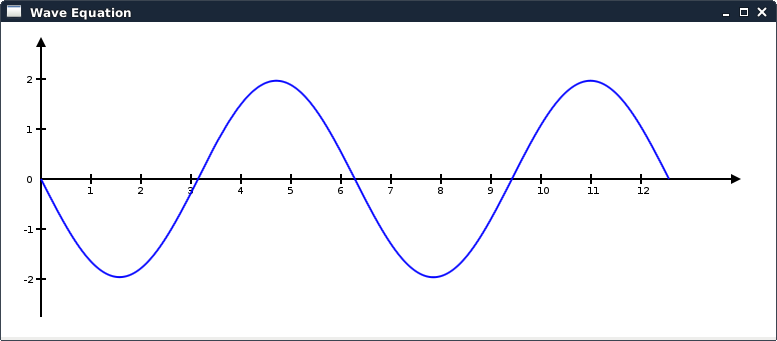
\includegraphics[width=0.9\textwidth]{pictures/gui}
	\caption{Graphical User Interface (GUI)}
	\label{fig:gui}
\end{figure}
% !TEX root = main.tex

\section{Test}
%manuelle Tests?
%Testskripte
%Vergleich von seriell und parallel

\subsection{manuelle Tests}
\subsection{automatisierte Tests}
\subsection{Auswertung der Tests}
% !TEX root = main.tex

\section{Fazit}
Zusammenfassend kann gesagt werden, dass die Parallelisierung der Wellensimulation das Potenzial zur Zeiteinsparung hat. Bei der Verwendung der zwei Softwarebibliotheken OpenMP und OpenMPI konnten positive als auch negative Verbesserungen beobachtet werden.
Der Einsatz von OpenMP brachte hierbei eine Performanceverbesserung. Diese offenbart sich mit einem Speedup von 1,08 zur Ausgangslösung. Die Verbesserung liegt jedoch niedriger als erwartet. Ein Grund dafür besteht in der geringen Rechenlast der Simulationsberechnung. Durchgeführte Versuche mit unnötigen Berechnungen die Rechenlast zu erhöhen haben bei der Problemsuche die Laufzeit-Performance verbessern können.
 
Die Umsetzung der Parallelisierung gestaltete sich außerdem mit OpenMP wesentlich einfacher als mit OpenMPI. Die Umsetzung mit OpenMPI hat, im Bezug dessen, ein Konzept zur Verteilung der Arbeitlast von Nöten gemacht. Dafür musste das passgenaue Senden und Empfangen von Nachrichten zwischen Threads implementiert werden. Dies erhöht die Komplexität des Code und trägt nicht zur Übersichtlichkeit bei. 

Ein weiterer Nachteil der umgesetzte Variante ist die Vergrößerung der Laufzeit der Simulation im Vergleich zur sequentiellen Variante. Der ermittelte Speedup von maximal 0,33 zeigt die Verschlechterung der Laufzeit auf. Diese Entwicklung widerspricht den Projektziel. Ein Grund für die zeitliche Verschlechterung liegt im Verteilungsaufwands des umgesetzten Master-Worker Konzepts. Dieser spielt hier als zeitlicher Kostenfaktor eine große Rolle und führt zu dem vorliegenden Ergebnis.
%Mehr eingehen auf Testwerte

\pagestyle{plain}
\bibliographystyle{plain}
\bibliography{bibliography}

%\section{Anhang}
%Verweis auf repository?

\end{document}
\grid
\grid
\grid
\grid
\grid
\grid
\grid
\grid
\grid
